
%% bare_conf.tex
%% V1.3
%% 2007/01/11
%% by Michael Shell
%% See:
%% http://www.michaelshell.org/
%% for current contact information.
%%
%% This is a skeleton file demonstrating the use of IEEEtran.cls
%% (requires IEEEtran.cls version 1.7 or later) with an IEEE conference paper.
%%
%% Support sites:
%% http://www.michaelshell.org/tex/ieeetran/
%% http://www.ctan.org/tex-archive/macros/latex/contrib/IEEEtran/
%% and
%% http://www.ieee.org/

%%*************************************************************************
%% Legal Notice:
%% This code is offered as-is without any warranty either expressed or
%% implied; without even the implied warranty of MERCHANTABILITY or
%% FITNESS FOR A PARTICULAR PURPOSE! 
%% User assumes all risk.
%% In no event shall IEEE or any contributor to this code be liable for
%% any damages or losses, including, but not limited to, incidental,
%% consequential, or any other damages, resulting from the use or misuse
%% of any information contained here.
%%
%% All comments are the opinions of their respective authors and are not
%% necessarily endorsed by the IEEE.
%%
%% This work is distributed under the LaTeX Project Public License (LPPL)Como somos conscientes de que 
%% ( http://www.latex-project.org/ ) version 1.3, and may be freely used,
%% distributed and modified. A copy of the LPPL, version 1.3, is included
%% in the base LaTeX documentation of all distributions of LaTeX released
%% 2003/12/01 or later.
%% Retain all contribution notices and credits.
%% ** Modified files should be clearly indicated as such, including  **
%% ** renaming them and changing author support contact information. **
%%
%% File list of work: IEEEtran.cls, IEEEtran_HOWTO.pdf, bare_adv.tex,
%%                    bare_conf.tex, bare_jrnl.tex, bare_jrnl_compsoc.tex
%%*************************************************************************

% *** Authors should verify (and, if needed, correct) their LaTeX system  ***
% *** with the testflow diagnostic prior to trusting their LaTeX platform ***
% *** with production work. IEEE's font choices can trigger bugs that do  ***
% *** not appear when using other class files.                            ***
% The testflow support page is at:
% http://www.michaelshell.org/tex/testflow/



% Note that the a4paper option is mainly intended so that authors in
% countries using A4 can easily print to A4 and see how their papers will
% look in print - the typesetting of the document will not typically be
% affected with changes in paper size (but the bottom and side margins will).
% Use the testflow package mentioned above to verify correct handling of
% both paper sizes by the user's LaTeX system.
%
% Also note that the "draftcls" or "draftclsnofoot", not "draft", option
% should be used if it is desired that the figures are to be displayed in
% draft mode.
%
\documentclass[conference]{IEEEtran}
% Add the compsoc option for Computer Society conferences.
%
% If IEEEtran.cls has not been installed into the LaTeX system files,
% manually specify the path to it like:
% \documentclass[conference]{../sty/IEEEtran}





% Some very useful LaTeX packages include:
% (uncomment the ones you want to load)


% *** MISC UTILITY PACKAGES ***
%
%\usepackage{ifpdf}
% Heiko Oberdiek's ifpdf.sty is very useful if you need conditional
% compilation based on whether the output is pdf or dvi.
% usage:
% \ifpdf
%   % pdf code
% \else
%   % dvi code
% \fi
% The latest version of ifpdf.sty can be obtained from:
% http://www.ctan.org/tex-archive/macros/latex/contrib/oberdiek/
% Also, note that IEEEtran.cls V1.7 and later provides a builtin
% \ifCLASSINFOpdf conditional that works the same way.
% When switching from latex to pdflatex and vice-versa, the compiler may
% have to be run twice to clear warning/error messages.


\usepackage[british,spanish]{babel}
\usepackage[utf8]{inputenc}



% *** CITATION PACKAGES ***
%
%\usepackage{cite}
% cite.sty was written by Donald Arseneau
% V1.6 and later of IEEEtran pre-defines the format of the cite.sty package
% \cite{} output to follow that of IEEE. Loading the cite package will
% result in citation numbers being automatically sorted and properly
% "compressed/ranged". e.g., [1], [9], [2], [7], [5], [6] without using
% cite.sty will become [1], [2], [5]--[7], [9] using cite.sty. cite.sty's
% \cite will automatically add leading space, if needed. Use cite.sty's
% noadjust option (cite.sty V3.8 and later) if you want to turn this off.
% cite.sty is already installed on most LaTeX systems. Be sure and use
% version 4.0 (2003-05-27) and later if using hyperref.sty. cite.sty does
% not currently provide for hyperlinked citations.
% The latest version can be obtained at:
% http://www.ctan.org/tex-archive/macros/latex/contrib/cite/
% The documentation is contained in the cite.sty file itself.






% *** GRAPHICS RELATED PACKAGES ***
%
\ifCLASSINFOpdf
  \usepackage[pdftex]{graphicx}
  % declare the path(s) where your graphic files are
  % \graphicspath{{../pdf/}{../jpeg/}}
  % and their extensions so you won't have to specify these with
  % every instance of \includegraphics
  \DeclareGraphicsExtensions{.pdf,.jpeg,.png}
\else
  % or other class option (dvipsone, dvipdf, if not using dvips). graphicx
  % will default to the driver specified in the system graphics.cfg if no
  % driver is specified.
  % \usepackage[dvips]{graphicx}
  % declare the path(s) where your graphic files are
  % \graphicspath{{../eps/}}
  % and their extensions so you won't have to specify these with
  % every instance of \includegraphics
  % \DeclareGraphicsExtensions{.eps}
\fi
% graphicx was written by David Carlisle and Sebastian Rahtz. It is
% required if you want graphics, photos, etc. graphicx.sty is already
% installed on most LaTeX systems. The latest version and documentation can
% be obtained at: 
% http://www.ctan.org/tex-archive/macros/latex/required/graphics/
% Another good source of documentation is "Using Imported Graphics in
% LaTeX2e" by Keith Reckdahl which can be found as epslatex.ps or
% epslatex.pdf at: http://www.ctan.org/tex-archive/info/
%
% latex, and pdflatex in dvi mode, support graphics in encapsulated
% postscript (.eps) format. pdflatex in pdf mode supports graphics
% in .pdf, .jpeg, .png and .mps (metapost) formats. Users should ensure
% that all non-photo figures use a vector format (.eps, .pdf, .mps) and
% not a bitmapped formats (.jpeg, .png). IEEE frowns on bitmapped formats
% which can result in "jaggedy"/blurry rendering of lines and letters as
% well as large increases in file sizes.
%
% You can find documentation about the pdfTeX application at:
% http://www.tug.org/applications/pdftex





% *** MATH PACKAGES ***
%
%\usepackage[cmex10]{amsmath}
% A popular package from the American Mathematical Society that provides
% many useful and powerful commands for dealing with mathematics. If using
% it, be sure to load this package with the cmex10 option to ensure that
% only type 1 fonts will utilized at all point sizes. Without this option,
% it is possible that some math symbols, particularly those within
% footnotes, will be rendered in bitmap form which will result in a
% document that can not be IEEE Xplore compliant!
%
% Also, note that the amsmath package sets \interdisplaylinepenalty to 10000
% thus preventing page breaks from occurring within multiline equations. Use:
%\interdisplaylinepenalty=2500
% after loading amsmath to restore such page breaks as IEEEtran.cls normally
% does. amsmath.sty is already installed on most LaTeX systems. The latest
% version and documentation can be obtained at:
% http://www.ctan.org/tex-archive/macros/latex/required/amslatex/math/





% *** SPECIALIZED LIST PACKAGES ***
%
%\usepackage{algorithmic}
% algorithmic.sty was written by Peter Williams and Rogerio Brito.
% This package provides an algorithmic environment fo describing algorithms.
% You can use the algorithmic environment in-text or within a figure
% environment to provide for a floating algorithm. Do NOT use the algorithm
% floating environment provided by algorithm.sty (by the same authors) or
% algorithm2e.sty (by Christophe Fiorio) as IEEE does not use dedicated
% algorithm float types and packages that provide these will not provide
% correct IEEE style captions. The latest version and documentation of
% algorithmic.sty can be obtained at:
% http://www.ctan.org/tex-archive/macros/latex/contrib/algorithms/
% There is also a support site at:
% http://algorithms.berlios.de/index.html
% Also of interest may be the (relatively newer and more customizable)
% algorithmicx.sty package by Szasz Janos:
% http://www.ctan.org/tex-archive/macros/latex/contrib/algorithmicx/




% *** ALIGNMENT PACKAGES ***
%
%\usepackage{array}
% Frank Mittelbach's and David Carlisle's array.sty patches and improves
% the standard LaTeX2e array and tabular environments to provide better
% appearance and additional user controls. As the default LaTeX2e table
% generation code is lacking to the point of almost being broken with
% respect to the quality of the end results, all users are strongly
% advised to use an enhanced (at the very least that provided by array.sty)
% set of table tools. array.sty is already installed on most systems. The
% latest version and documentation can be obtained at:
% http://www.ctan.org/tex-archive/macros/latex/required/tools/


%\usepackage{mdwmath}
%\usepackage{mdwtab}
% Also highly recommended is Mark Wooding's extremely powerful MDW tools,
% especially mdwmath.sty and mdwtab.sty which are used to format equations
% and tables, respectively. The MDWtools set is already installed on most
% LaTeX systems. The lastest version and documentation is available at:
% http://www.ctan.org/tex-archive/macros/latex/contrib/mdwtools/


% IEEEtran contains the IEEEeqnarray family of commands that can be used to
% generate multiline equations as well as matrices, tables, etc., of high
% quality.


%\usepackage{eqparbox}
% Also of notable interest is Scott Pakin's eqparbox package for creating
% (automatically sized) equal width boxes - aka "natural width parboxes".
% Available at:
% http://www.ctan.org/tex-archive/macros/latex/contrib/eqparbox/





% *** SUBFIGURE PACKAGES ***
%\usepackage[tight,footnotesize]{subfigure}
% subfigure.sty was written by Steven Douglas Cochran. This package makes it
% easy to put subfigures in your figures. e.g., "Figure 1a and 1b". For IEEE
% work, it is a good idea to load it with the tight package option to reduce
% the amount of white space around the subfigures. subfigure.sty is already
% installed on most LaTeX systems. The latest version and documentation can
% be obtained at:
% http://www.ctan.org/tex-archive/obsolete/macros/latex/contrib/subfigure/
% subfigure.sty has been superceeded by subfig.sty.



%\usepackage[caption=false]{caption}
%\usepackage[font=footnotesize]{subfig}
% subfig.sty, also written by Steven Douglas Cochran, is the modern
% replacement for subfigure.sty. However, subfig.sty requires and
% automatically loads Axel Sommerfeldt's\usepackage[british,spanish]{babel}
%\usepackage[utf8]{inputenc} caption.sty which will override
% IEEEtran.cls handling of captions and this will result in nonIEEE style
% figure/table captions. To prevent this problem, be sure and preload
% caption.sty with its "caption=false" package option. This is will preserve
% IEEEtran.cls handing of captions. Version 1.3 (2005/06/28) and later 
% (recommended due to many improvements over 1.2) of subfig.sty supports
% the caption=false option directly:
%\usepackage[caption=false,font=footnotesize]{subfig}
%
% The latest version and documentation can be obtained at:
% http://www.ctan.org/tex-archive/macros/latex/contrib/subfig/
% The latest version and documentation of caption.sty can be obtained at:
% http://www.ctan.org/tex-archive/macros/latex/contrib/caption/




% *** FLOAT PACKAGES ***
%
%\usepackage{fixltx2e}
% fixltx2e, the successor to the earlier fix2col.sty, was written by
% Frank Mittelbach and David Carlisle. This package corrects a few problems
% in the LaTeX2e kernel, the most notable of which is that in current
% LaTeX2e releases, the ordering of single and double column floats is not
% guaranteed to be preserved. Thus, an unpatched LaTeX2e can allow a
% single column figure to be placed prior to an earlier double column
% figure. The latest version and documentation can be found at:
% http://www.ctan.org/tex-archive/macros/latex/base/kile



%\usepackage{stfloats}
% stfloats.sty was written by Sigitas Tolusis. This package gives LaTeX2e
% the ability to do double column floats at the bottom of the page as well
% as the top. (e.g., "\begin{figure*}[!b]" is not normally possible in
% LaTeX2e). It also provides a command:
%\fnbelowfloat
% to enable the placement of footnotes below bottom floats (the standard
% LaTeX2e kernel puts them above bottom floats). This is an invasive package
% which rewrites many portions of the LaTeX2e float routines. It may not work
% with other packages that modify the LaTeX2e float routines. The latest
% version and documentation can be obtained at:
% http://www.ctan.org/tex-archive/macros/latex/contrib/sttools/
% Documentation is contained in the stfloats.sty comments as well as in the
% presfull.pdf file. Do not use the stfloats baselinefloat ability as IEEE
% does not allow \baselineskip to stretch. Authors submitting work to the
% IEEE should note that IEEE rarely uses double column equations and
% that authors should try to avoid such use. Do not be tempted to use the
% cuted.sty or midfloat.sty packages (also by Sigitas Tolusis) as IEEE does
% not format its papers in such ways.

%\usepackage[table]{xcolor}
\usepackage{todonotes}
%\usepackage{menukeys}

\usepackage{url}

% *** PDF, URL AND HYPERLINK PACKAGES ***
%
%\usepackage{url}
% url.sty was written by Donald Arseneau. It provides better support for
% handling and breaking URLs. url.sty is\usepackage[british,spanish]{babel}
%\usepackage[utf8]{inputenc} already installed on most LaTeX
% systems. The latest version can be obtained at:
% http://www.ctan.org/tex-archive/macros/latex/contrib/misc/
% Read the url.sty source comments for usage information. Basically,
% \url{my_url_here}.





% *** Do not adjust lengths that control margins, column widths, etc. ***
% *** Do not use packages that alter fonts (such as pslatex).         ***
% There should be no need to do such things with IEEEtran.cls V1.6 and later.
% (Unless specifically asked to do so by the journal or conference you plan
% to submit to, of course. )


% correct bad hyphenation here
\hyphenation{op-tical net-works semi-conduc-tor}

\usepackage{hyperref}
\begin{document}
%
% paper title
% can use linebreaks \\ within to get better formatting as desired
\title{Diseño curricular del``Desarrollo de apliaciones para la nube'' siguiendo las pautas ACM/IEEE CS2013: Un caso práctico en la Universidad de Las Palmas de GC}


% author names and affiliations
% use a multiple column layout for up to three different
% affiliations
\author{\IEEEauthorblockN{Francisca Quintana-Domínguez\\ y Carmelo Cuenca-Hernández}
\IEEEauthorblockA{Departamento de Informática y Sistemas\\
Universidad de Las Palmas de Gran Canaria\\
Las Palmas, Spain 35017\\
Email: fquintana@dis.ulpgc.es}
}

% conference papers do not typically use \thanks and this command
% is locked out in conference mode. If really needed, such as for
% the acknowledgment of grants, issue a \IEEEoverridecommandlockouts
% after \documentclass

% for over three affiliations, or if they all won't fit within the width
% of the page, use this alternative format:
% 
%\author{\IEEEauthorblockN{Michael Shell\IEEEauthorrefmark{1},
%Homer Simpson\IEEEauthorrefmark{2},
%James Kirk\IEEEauthorrefmark{3}, 
%Montgomery Scott\IEEEauthorrefmark{3} and
%Eldon Tyrell\IEEEauthorrefmark{4}}
%\IEEEauthorblockA{\IEEEauthorrefmark{1}School of Electrical and Computer Engineering\\
%Georgia Institute of Technology,
%Atlanta, Georgia 30332--0250\\ Email: see http://www.michaelshell.org/contact.html}
%\IEEEauthorblockA{\IEEEauthorrefmark{2}Twentieth Century Fox, Springfield, USA\\
%Email: homer@thesimpsons.com}
%\IEEEauthorblockA{\IEEEauthorrefmark{3}Starfleet Academy, San Francisco, California 96678-2391\\
%Telephone: (800) 555--1212, Fax: (888) 555--1212}
%\IEEEauthorblockA{\IEEEauthorrefmark{4}Tyrell Inc., 123 Replicant Street, Los Angeles, California 90210--4321}}




% use for special paper notices
%\IEEEspecialpapernotice{(Invited Paper)}




% make the title area
\maketitle


\begin{abstract}
%\boldmath
Este artículo describe la puesta en marcha de la asignatura ``Desarrollo de aplicaciones para la nube'' en el contexto del Experto Universitario de Virtualización y Computación en la nube impartido en la Universidad de Las Palmas de Gran Canaria.
La asignatura, de 6 créditos ECTS, está planificada según las pautas del EEES donde el proceso de enseñanza-aprendizaje está centrado en el estudiante y sigue al máximo la directriz de aprender haciendo.
Para ello, los estudiantes utilizan laboratorios virtuales construidos con servicios en la nube proporcionados por proveedores públicos.
Los contenidos han sido diseñados siguiendo la guía curricular de la ACM/IEEE (CS2013).

\end{abstract}
% IEEEtran.cls defaults to using nonbold math in the Abstract.
% This preserves the distinction between vectors and scalars. However,
% if the conference you are submitting to favors bold math in the abstract,
% then you can use LaTeX's standard command \boldmath at the very start
% of the abstract to achieve this. Many IEEE journals/conferences frown on
% math in the abstract anyway.

% no keywords




% For peer review papers, you can put extra information on the cover
% page as needed:
% \ifCLASSOPTIONpeerreview
% \begin{center} \bfseries EDICS Category: 3-BBND \end{center}
% \fi
%
% For peerreview papers, this IEEEtran command inserts a page break and
% creates the second title. It will be ignored for other modes.
\IEEEpeerreviewmaketitle


% El trabajo describe el diseño curricular y la experiencia de impartición de una asignatura  denominada “Desarrollo de aplicaciones para la nube” dentro de un curso experto universitario.
% La temática del trabajo encaja por tanto perfectamente dentro de la categoría “Métodos y Casos en Educación en Informática”.
% El artículo está bien redactado y se lee con facilidad. La contribución del trabajo desde el punto de vista científico no está del todo claro.
% El uso de servicios como Amazon Web Service o  Google Cloud Platform no suele ser habitual en cursos universitarios y la descripción de una experiencia de uso en este contexto puede ser de interés para la comunidad.
% Sin embargo gran parte del documento se dedica a describir en detalle el diseño de los distintos bloques temáticos de la asignatura,
% razonando la elección de los frameworks y servicios a utilizar durante el curso.

% La experiencia concreta de los alumnos y las actividades de aprendizaje realiza! das son presentadas a un menor nivel de detalle.
% Por ejemplo: ¿en qué consistieron exactamente los trabajos y proyectos de los alumnos? ¿cuáles fueron las actividades concretas a desarrollar?
% ¿trabajaron en grupos o de forma individual? Las opciones de evaluación tampoco aparecen claramente explicadas.
% Se entiende por las conclusiones que existieron dos modalidades, tradicional y "eEvaluación" (¿no presencial?), aunque las diferencias entre ambas no son explicadas.
% Las conclusiones que pueden ser más interesantes para otros diseñadores instruccionales que se planteen diseñar cursos similares son aquellas relacionadas con la tecnología,
% sin embargo éstas son presentadas a un nivel muy general, con poca información sobre los puntos fuertes y débiles observados.
% Los parámetros utilizados para estimar el éxito del curso (estudiantes matriculados, tasas bajas de matrículas) podrían ser discutibles.
% El título de la referencia 8 aparece en mayúsculas.

\section{Introducción}
% no \IEEEPARstart

La Universidad de Las Palmas de Gran Canaria (ULPGC) en España imparte desde el
año 2009 la titulación oficial de Grado en Ingeniería Informática (GII). Una
titulación oficial está caracterizada por el carácter nacional y la
homogeneidad de la misma, con independencia del centro universitario
donde sea impartida. Esta homogeneidad, necesaria por una parte
para el reconocimiento nacional del título, también implica falta de
flexibilidad para adaptar las materias impartidas a las nuevas demandas de la
sociedad. La ULPGC ofrece
una oferta complementaria de títulos propios de Experto Universitario para
facilitar la adecuación a las nuevas tecnologías tanto de los recién titulados
y la especialización de los
profesionales ya titulados.

La computación en la nube (\textit{Cloud Computing}) \cite{Buyya:2013}, y dentro
de ésta la
infraestructura como
un servicio (\textit{Infraestructure as a Service o IaaS})
y 
la plataforma como un servicio (\textit{Platform as a Service o PaaS})
\cite{Carlson:2013},
constituyen un bloque temático cada vez más demandado por los estudiantes y
profesionales de las Tecnologías de la Información y de las Comunicaciones
(TIC), lo cual además coincide con temas de interés de la guía curricular de la ACM/IEEE CS2013 \cite{acm:2013}.




Dado
el carácter novedoso de estas materias, que poca cabida tuvieron en la
titulación de GII, la ULPGC empezó a impartir enel curso 2013/14 el título propio de Experto Universitario en
Virtualización y Computación en la Nube (EUVCN)\footnote{Experto Universitario en Computación en la Nube,
\url{http://eii.ulpgc.es/experto\_cloud}}. Este título
propio, de 24
créditos ECTS,
está estructurado  en 4 asignaturas de 6 créditos:
``Virtualización'',
``Clusters de computadores y almacenamiento distribuido'', ``Desarrollo de
aplicaciones para la nube'' (DAN) e ``Infraestructuras tecnológicas para la
computación en la nube'' y se cursa durante un año académico.

La asignatura  incluye dos
bloques temáticos: el primero dedicado a las IaaS públicas y el segundo,
centrado en el desarrollo de aplicaciones que aprovechen las IaaS públicas
utilizando PaaS. Este carácter de distribuido (``o en la nube'') de las
materias a tratar en la asignatura hace que la utilización de
laboratorios virtuales (LVs) \cite{Zhang:2010} sea una necesidad implícita y un
sin sentido el
empleo de
laboratorios convencionales (LCs), más allá de proveer a los estudiantes de un puesto de trabajo
ofimático.





Este artículo describe la planificación y puesta en marcha de la asignatura
DAN del EUVCN. En  la sección \ref{sec:contenidos_educativos} se describen los
contenidos educativos desarrollados, los cuales motivan la necesidad de la
utilización de un LV para la formación práctica. En la sección
\ref{sec:laboratorios_virtuales} se trata el uso de los servicios de
\textit{Amazon Web Services} \cite{AWS:2011} y de \textit{Heroku}
\cite{Heroku:2013} para conformar el laboratorio
virtual de la asignatura. A continuación, en la sección \ref{sec:eValuacion}
se describe el procedimiento de eEvaluación \cite{Moral2013} como una acción más para facilitar el proceso de enseñanza aprendizaje. Finalmente, en la sección
\ref{sec:conclusiones} se establecen las conclusiones de este caso de uso de
educación en Informática.

El término computación en la nube aparece en la curricula ACM/IEEE CS2013 en el área de conocimiento de computación paralela y distribuida (\textit{Parallel and Distributed Computing} )
como una unidad de conocimiento (\textit{Knowledge Unit}) opcional y concluye con 5 resultados del aprendizaje.
Esta asignatura contiene los resultados de aprendizaje (\textit{Learning Outcome}) \#1 y \#4 de la propuesta curricular: \#1 Analizar la importancia de la elasticidad y el manejo de recursos en la computación en la nube
(\textit{Discuss the importance of elasticity and resource management in cloud computing.}) y
\#4 Desplegar una aplicación que use recursos de infraestructura en la nube para cómputo o datos
(\textit{Deploy an application that uses cloud infrastructure for computing and/or data resources}).
A tener en cuenta, es que resulta imposible plantear una asignatura de infraestructuras públicas y desarrollo de aplicaciones sin cubrir
otras áreas o unidades de conocimiento de los planes de estudio, pero este artículo está centrado en los tópicos relacionados con la computación en la nube.

% An example of a floating figure using the graphicx package.
% Note that \label must occur AFTER (or within) \caption.
% For figures, \caption should occur after the \includegraphics.
% Note that IEEEtran v1.7 and later has special internal code that
% is designed to preserve the operation of \label within \caption
% even when the captionsoff option is in effect. However, because
% of issues like this, it may be the safest practice to put all your
% \label just after \caption rather than within \caption{}.
%
% Reminder: the "draftcls" or "draftclsnofoot", not "draft", class
% option should be used if it is desired that the figures are to be
% displayed while in draft mode.
%
%\begin{figure}[!t]
%\centering
%\includegraphics[width=2.5in]{myfigure}
% where an .eps filename suffix will be assumed under latex, 
% and a .pdf suffix will be assumed for pdflatex; or what has been declared
% via \DeclareGraphicsExtensions.
%\caption{Simulation Results}
%\label{fig_sim}
%\end{figure}

% Note that IEEE typically puts floats only at the top, even when this
% results in a large percentage of a column being occupied by floats.


% An example of a double column floating figure using two subfigures.
% (The subfig.sty package must be loaded for this to work.)
% The subfigure \label commands are set within each subfloat command, the
% \label for the overall figure must come after \caption.
% \hfil must be used as a separator to get equal spacing.
% The subfigure.sty package works much the same way, except \subfigure is
% used instead of \subfloat.
%
%\begin{figure*}[!t]
%\centerline{\subfloat[Case I]\includegraphics[width=2.5in]{subfigcase1}%
%\label{fig_first_case}}
%\hfil
%\subfloat[Case II]{\includegraphics[width=2.5in]{subfigcase2}%
%\label{fig_second_case}}}
%\caption{Simulation results}
%\label{fig_sim}
%\end{figure*}
%
% Note that often IEEE papers with subfigures do not employ subfigure
% captions (using the optional argument to \subfloat), but instead will
% reference/describe all of them (a), (b), etc., within the main caption.


% An example of a floating table. Note that, for IEEE style tables, the 
% \caption command should come BEFORE the table. Table text will default to
% \footnotesize as IEEE normally uses this smaller font for tables.
% The \label must come after \caption as always.
%
%\begin{table}[!t]
%% increase table row spacing, adjust to taste
%\renewcommand{\arraystretch}{1.3}
% if using array.sty, it might be a good idea to tweak the value of
% \extrarowheight as needed to properly center the text within the cells
%\caption{An Example of a Table}
%\label{table_example}
%\centering
%% Some packages, such as MDW tools, offer better commands for making tables
%% than the plain LaTeX2e tabular which is used here.
%\begin{tabular}{|c||c|}
%\hline
%One & Two\\
%\hline
%Three & Four\\
%\hline
%\end{tabular}
%\end{table}


% Note that IEEE does not put floats in the very first column - or typically
% anywhere on the first page for that matter. Also, in-text middle ("here")
% positioning is not used. Most IEEE journals/conferences use top floats
% exclusively. Note that, LaTeX2e, unlike IEEE journals/conferences, places
% footnotes above bottom floats. This can be corrected via the \fnbelowfloat
% command of the stfloats package.

\section{Contenidos educativos \label{sec:contenidos_educativos}}

La asignatura ``Desarrollo de aplicaciones para la nube'' (DAN) tiene 6 créditos
ECTS y sus objetivos son aprender a desplegar y migrar aplicaciones a la
nube y a desarrollar aplicaciones para la nube.

Para poder alcanzar estos objetivos es
imprescindible  manejar las infraestructuras tecnológicas de los
proveedores públicos de servicios en la nube. Dado que el estudiante de un curso de
experto universitario demanda ``aprender haciendo'' desde las primeras
horas de docencia, es necesario seleccionar
tempranamente un proveedor de servicios en la nube para ejemplificar los contenidos a
presentar.

Internet
está llena de enlaces y anuncios de proveedores de infraestructuras públicas
como un servicio, anuncios de los más grandes y populares como \textit{Amazon
Web Service} (AWS), \textit{Google Cloud Platform} o \textit{Windows Azure} (por
citar sólo a algunos) y también incluso anuncios de proveedores locales geográficamente.
La elección realizada para DAN fue
AWS, por ser una plataforma consolidada, con excelente documentación (incluso
existen algunos libros de texto dedicados a su estudio); AWS también es el
proveedor de servicios que aglutina una mayor variedad de servicios bajo un mismo entorno, y  proporciona servicios a
otros proveedores de infraestructura. Además dota  con becas de 100\$ para el
para el uso de sus infraestructura a  los estudiantes de cursos universitarios
donde enseñen AWS.

Los servicios de AWS seleccionados como contenidos educativos están relacionados
con diferentes temáticas:
servicios de computación (\textit{Elastic Cloud Computing} o EC2)
\cite{{Vliet:2011}},
servicios de almacenamiento  (\textit{Simple Storage Service} o S3),
red de entrega de contenidos (Cloudfront),
colas de desacoplo (\textit{Simple Queue Services} o SQS), balanceo elástico de
carga (\textit{Elastic Load Balancer} o ELB), bases de datos relacionales (RDS) y bases de datos
no relaciones (SimpleDB) \cite{Chaganti:2010}.

La interacción de los estudiantes con los servicios remotos proporcionados con
AWS tiene lugar desde equipos locales utilizando un \textit{Application
Programming Interface} (API). Esta API está desarrollada para casi todos los
lenguajes más comunes como PHP, Java,
Javascript \dots y también otros menos populares Python o Ruby \cite{Ruby:2013}.
La elección de uno u otro, podría no ser relevante de no considerar el requisito
de unificar el lenguaje de programación
a usar tanto en este primer bloque temático de uso de servicios de
infraestructura con el segundo bloque temático. Con este objetivo en mente, el
lenguaje de programación seleccionado fue Ruby.

Uno de los escenarios laborales más usuales consistirá en migrar un servicio a la nube.
Las pequeñas y medianas empresas demandan migrar una aplicación local a la nube.
Ya no solámente servicios tradicionales como el correo electrónico, sino también sus propias aplicaciones.
Por este motivo, la parte práctica de la utilización de los servicios de computación EC2
consistió en migrar una aplicación local ya desarrollada a la nube teniendo en
cuenta las particularidades de la aplicación \cite{Reese:2013, Barr:2010}. Una
vez movida la aplicación, la modificamos  para que sea escalable
horizontalmente y poder usar los servicios de autoescalado de AWS, balanceo de
carga ELB y RDS.
El escalado horizontal consiste en el despliegue de máquinas clones con las mismas características  como respuesta a la ocurrencia de eventos predefinidos
(peticiones http, carga de la CPU \dots). La otra opción para responder a aumentos de demanda es el escalado vertical donde las características de la máquina escala a una de mayor prestaciones.

\begin{figure}[!t]
\centering
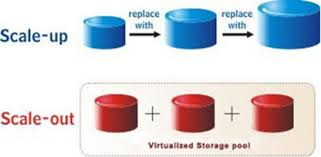
\includegraphics[width=\columnwidth]{scale.jpeg}
\caption{Escalado vertical frente escalado horizontal.}
\label{fig:console}
\end{figure}

La infraestructura virtual desplegada es estresada mediante
un patrón de alta y baja carga definido con JMeter \cite{{Erinle:2013}} para
comprobar la elasticidad de los servidores del sitio, provisonando servidores cuando aumenta la demanda y reduciendo el número de servidores cuando disminuye.


Un componente básico de la nube lo forman los sistemas de almacenamiento distribuidos. En este tema los estudiantes realizan programas para subir y descargar
ficheros al S3 de AWS utilizando credenciales de seguridad. También
estudian y practican
con la alta disponibilidad de los datos utilizando Cloudfront.

El desacoplo de tareas con colas permite adaptar el flujo de un proceso  a los
recursos disponibles. El desarrollo de una aplicación de \textit{scrapping}
de imágenes de una dirección de web para construir un mosaico con las
imágenes escaladas sirve de motivación para desacoplar las tareas
(almacenamiento de la url, análisis de su contenido, descarga de las imágenes
al S3, escalado y construcción del mosaico). Los datos o referencias a datos a
cada una de las tareas son encolados y desencolados en el SQS de AWS. En este
punto los estudiantes utilizan el servicio de base de datos no relacional
SimpleDB de AWS para almacenar los datos persistentes de la aplicación.


El segundo bloque temático de la asignatura trata sobre el desarrollo de aplicaciones para la
nube. El primer tema presenta las diferencias entre el desarrollo de una
aplicación web y el desarrollo de una aplicación para la nube
\cite{Heroku:2013,Wilder:2012}. La elección de un PasS para ``aprender
haciendo'' (y ``enseñar haciendo'') fija la selección concreta
de los LVs. En el momento de la confección de los contenidos, dos PaaS's
(Google App Engine \cite{Severance:2009} y Heroku) lideraban el mercado de las
plataformas como servicio. Google App Engine utilizaba como único lenguaje de
programación Python. Heroku es un PaaS construido sobre el IaaS de Amazon y estaba
orientado inicialmente a facilitar el despliegue de  aplicaciones escritas
en el framework de aplicaciones Ruby on Rails (RoR) \cite{Hartl:2012} (ahora
Heroku es políglota y permite el despliegue de aplicaciones en PHP, Java,
y otros lenguajes). RoR es un framework consolidado de desarrollo, utilizado por ejemplo en
las aplicaciones Twitter y GitHub. Todo esto, más la existencia de gemas (biblioteca de funciones y comandos de consola) para
facilitar el uso del manejo de las infraestructuras de AWS en RoR, y la
disponibilidad de una capa gratuita en Heroku para el despliegue de las
aplicaciones, condicionó la elección de Heroku como PaaS y RoR como framework de
programación.

Los contenidos de este bloque están centrados en el desarrollo de aplicaciones escalables horizontalmente, alta disponibilidad y alto rendimiento.
Los temas a tratar son las aplicaciones sin estado, procesos en \textit{background}, subidas de ficheros asíncronas,
manejo de \textit{cache} y  de servidores de \textit{cache},
gestión de ficheros de \textit{logs} y utilización de paneles profesionales de gestión de aplicaciones.

\todo{A}
El éxito de una aplicación para la nube depende de muchos factores (que muchas veces no tienen que ver con el diseño tecnológico).
Uno de ellos es la experiencia del usuario y más concrétamente el tiempo de respuesta.
En aplicaciones con el requisito de alta disponibilidad y alto rendimiento, el uso efectivo de un mecanismo de \textit{cache} resulta imprescindible para proporcionar la experiencia de ``tiempo real'' a los usuarios.
La utilización de \textit{cache} implica tener en cuenta la seguridad de los datos ya almacenados de manera que no puedan ser accedidos por usuarios no autorizados.
Los estudiantes tratan estos tópicos configurando inicialmente un servidor local de \textit{MemCached} y luego optimizan partes de una aplicación ya desarrollada mediante las técnicas que proporciona Ruby on Rails de
\textit{page chaching} y \textit{fragment caching}. En una segunda parte, mueven la aplicación y el servidor de \textit{MemCached} a la plataforma Heroku.


\todo{A}
Una aplicación para la nube casi con toda seguridad utilizará procesos en \textit{background}. El trabajo concreto desarrollado por los estudiante fue la creación de las imágenes  miniatura
\textit{thumbnails} de imágenes subidas con anterioridad, para ello fue necesario proveer a la aplicación de un servidor de \textit{Redis} para guardar los datos específicos del trabajo en 
\textit{background}. Los dos casos de provisionamiento: la instalación y configuración de un servidor local de \textit{Redis} y la utilización de un \textit{add-on} de Heroku son estudiados.
La gestión de  procesos en \textit{background} implica la utilización de recursos virtuales en la plataforma donde está desplegada la aplicación para la nube,
el estudiante debe configurar el número mínimo y máximo de procesos en \textit{background} y calcular el coste económico de los mismos.
 
\todo{A}
Los ficheros de \textit{logs} proporcionan información de la utilización de la aplicación. En una aplicación no escalable la información de \textit{logs} está en ficheros generalmente locales al servidor.
Las configuraciones autoescalables requieren del patrón de \textit{stateless} y ello implica establecer una gestión externa de la información de \textit{logs}.
Utilizamos el \textit{add-on} ``PaperClip'' de Heroku que proporciona el servicio de externalización de \textit{logs}, los estudiantes emplean la consola para clasificar la información,
realizar búsquedas, establecer reglas; también calculan el coste a pagar al proveedor del servicio y aprenden el establecimiento de alarmas.


El uso de los servicios ofertados por los
proveedores públicos implica ser capaz de realizar una previsión del coste de
utilización de dichos servicios. Por eso en la asignatura también trabajamos en la
realización de presupuestos para uso de los servicios públicos, como medio
también de decidir cuál de los proveedores ofrece una mejor relación
precio/servicios en determinados escenarios.



\section{Laboratorios virtuales \label{sec:laboratorios_virtuales}}

En ciencias de la computación, el término ``virtual'' significa que no es ``real''.
En el caso de la computación en la nube y más concretamente con las IaaS y PaaS, el término virtual y la realidad son indistinguible.
No existe la opción de un laboratorio real (LR) diferente al virtual. En cualquier caso, la utilización de un LR o LV no excluye la necesidad de un computador personal para realizar la conexión al mismo.

El diseño del laboratorio para el estudio de la IaaS  puede realizarse
o bien dotándose de los servidores físicos y del software necesario tipo \textit{OpenStack} \cite{Pepple:2011} u \textit{Open Nebula}, o bien utilizando infraestructuras externas.
El primer caso, requiere un desembolso económico en estos días inabordable para un centro universitario.
La alternativa de construir con máquinas virtuales en un computador personal IaaS compromete el estudio de la escalabilidad horizontal,
además de  alejar al estudiante de la materia de la asignatura dedicándole a tareas avanzadas de administración de sistemas.
Es por ello que el sistema de ``pago por uso'' constituyó la única alternativa real viable.

\todo{C}
La mejor opción para los laboratorios la constituyó AWS por diversos motivos.
AWS proporciona una cantidad ingente de material libre: vídeos, tutoriales, documentación, cursos que cubren temas básicos y también avanzados.
AWS permite el uso de sus servicios a través de una consola web (ver Fig.~\ref{fig:console}), lo que proporciona una  manera sencilla de presentar
los servicios antes de empezar con temas más avanzados de administración con líneas de comando o programación.
Además AWS dispone de un programa educativo de becas orientadas a la promoción de cursos realizados dentro del entorno universitario con unas cuantías más que suficientes
para la realización de las prácticas planteadas, el 80\% de los estudiantes no consumió el total de la beca, y el 20\% restante que lo consumió fue por causas ajenas al curso
(descuidos a la hora de apagar las máquinas o publicar las claves privadas para el acceso a los recursos).
El requisito solicitado por Amazon para disponer de las becas para los alumnos es tan simple como rellenar un formulario con los datos del curso (universidad, contenidos, fechas de impartición).
Estas becas no incluyen todos los servicios, por ejemplo, es posible utilizar con la beca de manera gratuita instancias \textit{Small} de EC2, pero no en cambio lanzar instancias \textit{Large} de EC2.

\begin{figure}[!t]
\centering
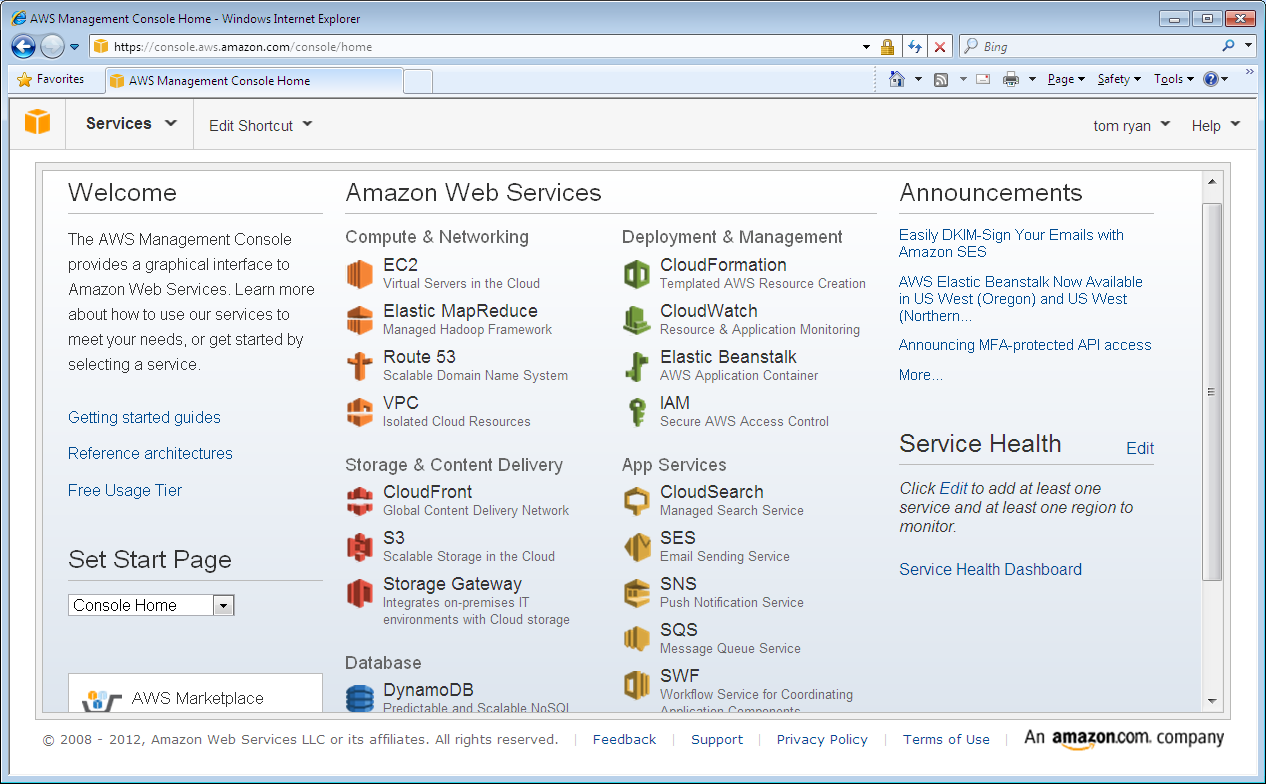
\includegraphics[width=\columnwidth]{aws_management_console_home.png}
\caption{Consola web de acceso a Amazon Web Services.}
\label{fig:console}
\end{figure} 

Para el bloque temático de desarrollo de aplicaciones, los estudiantes contaron con computadores personales y software de desarrollo (Software Libre).
La parte más relevante de este bloque es el despliegue continuo de las aplicaciones a la nube; Heroku la plataforma elegida para conformar el LV proporciona
el sistema de integración continuo entre los entornos de desarrollo y producción necesario en las metodologías iterativas de desarrollo.
Una sofisticada consola web (ver Fig.~\ref{fig:heroku}) permite añadir recursos a nuestra aplicación,
sin necesidad de desplegar las infraestructuras reales que los proporcionen.

Otra vez, al igual que con AWS, la capa gratuita proporcionada por Heroku es suficiente para el desarrollo de los objetivos de la asignatura lo que implica un ahorro en costes que repercute directamente en el estudiante.

\begin{figure}[!t]
\centering
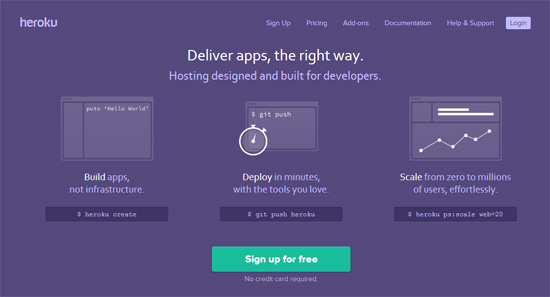
\includegraphics[width=\columnwidth]{heroku.jpeg}
\caption{Consola web de acceso al PaaS Heroku.}
\label{fig:heroku}
\end{figure}




\section{eEvaluación
\label{sec:eValuacion}}

La asignatura presentada está contextualizada en un curso de experto universitario cuyos contenidos versan acerca de la ``nube''.
Las características de la materia hacen que la manera adecuada de evaluación sean las evidencias obtenidas con la realización de los trabajos de cursos y proyectos propuestos.

Además de la utilización de una plataforma basada en Moodle para la distribución del material, la comunicación vía correos electrónicos y foros, y la entrega de documentación al profesor,
los LVs posibilitan la corrección remota de estos trabajos. Por ejemplo, el manejo de identidades de AWS permite que un estudiante habilite el acceso a los profesores a las infraestructuras a su cargo,
con lo cual estos pueden evaluar de manera remota los proyectos realizados.
Un estudiante puede planificar un aumento de demanda de un sitio web desplegado y configurar una alarma automática para este evento,
de manera que avise por correo electrónico o SMS al profesor de que puede ingresar para 
comprobar el correcto funcionamiento de las infraestructuras.


Por otro lado, se fomenta la utilización de repositorios en la nube para el código desarrollado, la definición de grupos de colaboración y el uso de PaaS, permite a los profesores la evaluación remota de las aplicaciones realizadas.
Los repositorios remotos permiten a los profesores clonar las aplicaciones para inspeccionar la calidad del código desarrollado y
la ejecución de una batería de pruebas sobre el código permite la comprobación de la correctitud del mismo. 

\todo{B}
En este contexto, entendemos por trabajos de curso modificaciones propuestas por los profesores de los ejemplos prácticos desarrollados durante las sesiones presenciales y que no requieren
de una gran dedicación temporal.
Estos trabajos de cursos fomentan la autonomía profesional ya que
el estudiante  busca individualmente la solución a los trabajos planteados, acostumbrándose a manejar y valorar la información proporcionada por
los proveedores y a enfrentarse a las nuevas circunstancias que aparezcan.

\todo{B}
Así para la temática de autoescalado de las máquinas virtuales, el trabajo de curso consistió en cambiar las alarmas del servicio \textit{CloudWatch} para que la provisión de infraestructura
no ocurriera tal y como los profesores la presentaron mediante un pico de la utilización de la CPU,
sino a una hora determinada (simulando un inicio de un jornada laboral, un comienzo de un evento concreto \dots). Los estudiantes, en el caso del S3, tuvieron que escribir una versión simplificada
de la orden \texttt{rsync} de Linux para sincronizar un respositorio local con un \textit{bucket} en el S3 de AWS.
 
\todo{B}
Dos fueron los proyectos planteados, uno para cada temática de la asignatura.

\todo{B}
El primero aglutina en un único trabajo todos los servicios de AWS estudiados. La aplicación dada una \textit{url}
(en la práctica utilizamos las direcciones de diarios digitales) determinaba qué palabras (excluidas preposiciones y artículos) y con qué frecuencia
se utilizaban en los titulares de las noticias. La figura \ref{fig:trabajo} ayuda a entender el proyecto.
Hay cuatro colas. Un primer script que simplemente añade la \textit{url} de partida a la cola de \textit{urls}.
Un proceso que recoge los mensajes en este cola y descarga la página html al S3 y genera dos mensajes con la información de la localización
de la página: una para la cola de títulos y otro para la cola  de \textit{crawler}.
Otro proceso  recoge los mensajes en la cola de titulos y crea otro fichero en el S3 con texto plano con el contenido de los títulos y añade un mensaje a la cola de contar palabras.
Otro proceso más paralelamente al anterior coge los datos la cola de \textit{crawler} y busca \textit{urls} relativas al sitio y las añade a la cola de \textit{urls}.
Un último proceso toma el texto plano del fichero en el S3 indicado en el mensaje del la cola de contar palabras y registra en simpleDB la utilización de las palabras.

En el segundo proyecto, los estudiantes desarrollaron una aplicación web (la propuesta fue una aplicación de zapatos) a desplegar en Heroku.
Tenían que utilizar procesos en \textit{background} y técnicas de \textit{cache} a la vez que el servicio de almacenamiento del S3 para la gestión de la subida de ficheros.


\todo{Mentira pero...}
La elección de Ruby como lenguaje de programación y Ruby on Rails como framework de desarollo tiene una ventaja añadida cara a realizar la eEvaluación de los trabajos y proyectos del curso.
Ruby y Ruby on Rails incluyen frameworks de prueba (TestUnit, RSpec, Cucumber, \dots...) que permiten fácilmente el diseño de pruebas por parte del profesorado para comprobar la correción de los desarrollos,
y llegado el caso, incluso a la automatización de los mismos.


\begin{figure}[!t]
\centering
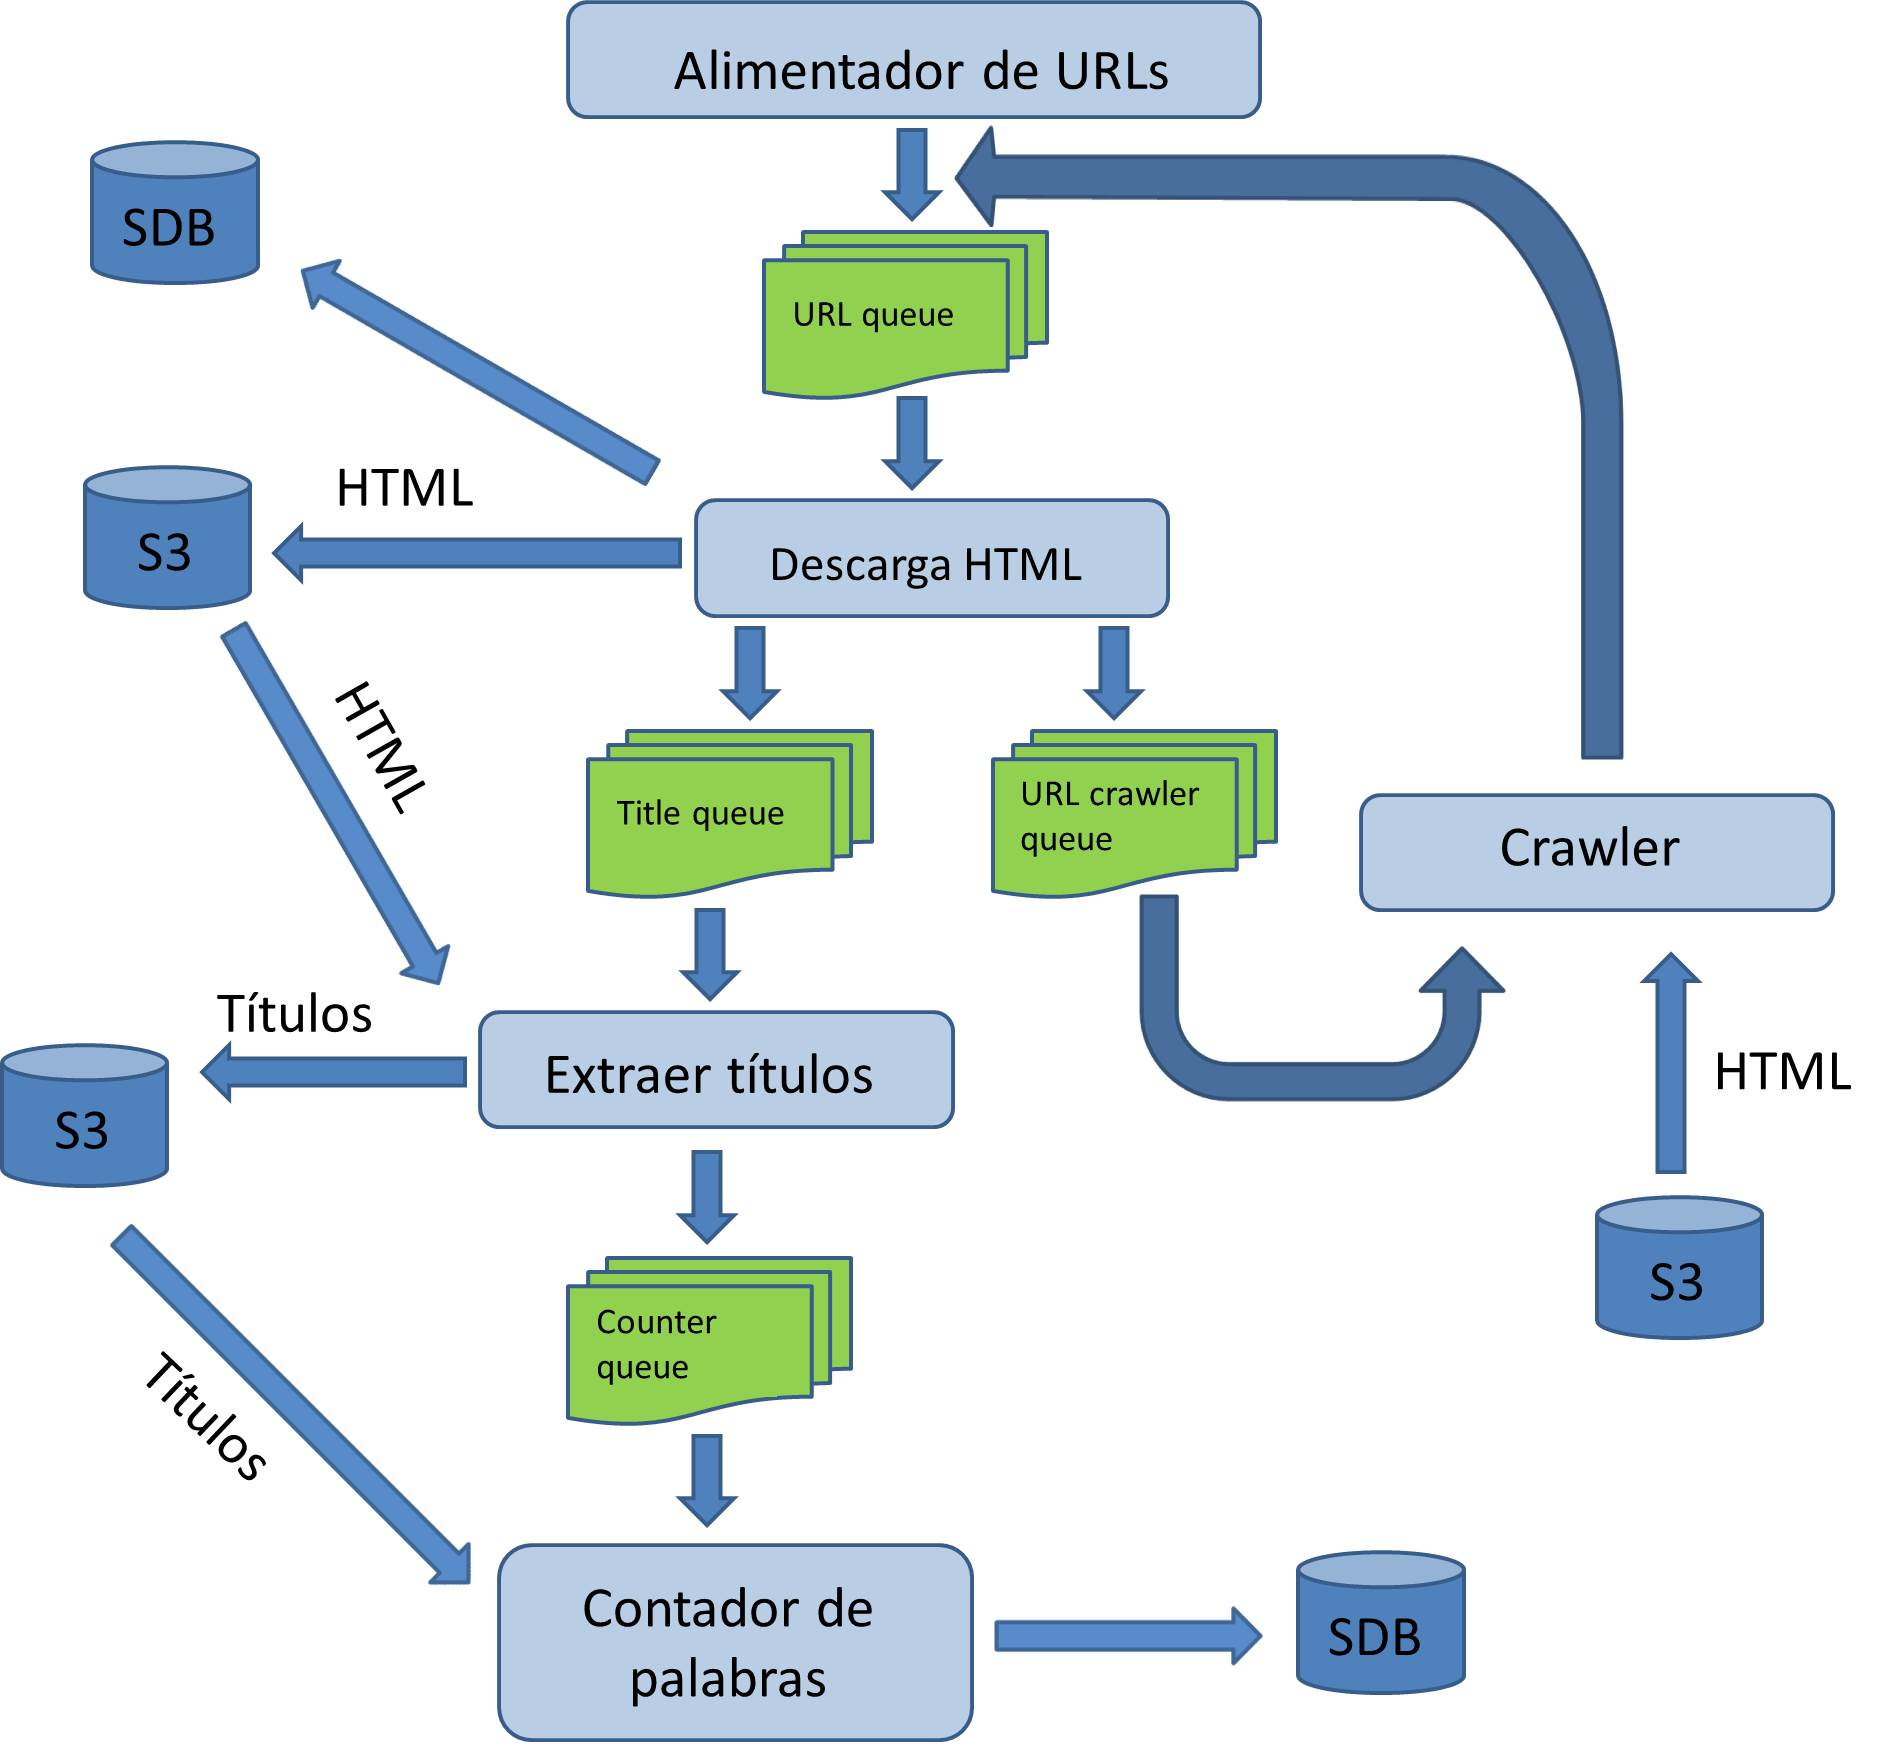
\includegraphics[width=\columnwidth]{Homework_sqs_sdb.jpeg}
\caption{Una propuesta de proyecto fin de curso para los servicios AWS.}
\label{fig:trabajo}
\end{figure}

\section{Conclusiones \label{sec:conclusiones}}

El éxito de una propuesta de un título de Experto Universitario pueden medirse
en primera aproximación por el baremo de tener un número suficiente de
estudiantes matriculados que posibiliten su impartición. En el caso presentado
de EUVCN, el número de estudiantes matriculados durante el curso 2013/2014
(primer año de impartición) ha sido  de 19 (el número mínimo necesario para
comenzar la impartición fue definido en
10 y  el número máximo de plazas ofertadas eran 20) de los cuales finalizaron
18. Otra
segunda medida y también importante, lo constituyen las encuestas de
satisfacción al estudiante. Éstas son organizadas por la ULPGC para cada uno de los cursos que imparte y los resultados son publicados en el siguiente curso académico.

Un factor que también concluimos como determinante para el éxito de la
propuesta realizada es haber mantenido las tasas de matrículas lo más bajas
posibles. De hecho, las tasas de matrícula del EUVCN están entre las más bajas
para cursos técnicos de estas características impartidos en la ULPGC. Sin duda
alguna, la utilización de recursos virtuales, más allá incluso de los
laboratorios virtuales, con uso de infraestructuras como un servicio en la
nube, supuso un ahorro económico sustancial que tuvo su reflejo en la tasas de
matrícula. También la adecuación de las tecnologías a desarrollar en la asignatura a
las infraestructuras o plataformas para las que se disponía, o bien de una
capa gratuita de servicio o de becas, contribuyó a ello.

El perfil de los estudiantes matriculados estuvo repartido entre un
50\% de egresados con más de 15 años transcurridos desde la obtención de la
titulación y un 50\% de recién titulados.
El primer grupo necesitó apoyo específico para actualizarse en los fundamentos
de la materia a cursar, ya que éstos no habían sido objeto de estudio durante su
formación ni durante su ejercicio profesional (fundamentos como lenguajes
dinámicos, tecnologías de desarrollo web y metodologías recientes de ingeniería
del software). Este apoyo durante la impartición de las horas presenciales
consistió en la presencia de otro profesor (además del ponente) para resolver
las dificultades del estudiante para seguir la docencia, además de apoyos con
tutorías y diálogos virtuales a través de una plataforma digital proporcionada
por el centro basada en Moodle.

Todos los estudiantes apreciaron la metodología de enseñanza ``aprender
haciendo'', donde los contenidos fueron desarrollados principalmente mediante
supuestos prácticos y prácticas en laboratorios virtuales. El uso de los
laboratorios virtuales (provisionados por Amazon) desde la primera sesión de la
asignatura confirió a ésta una cercanía al mundo real de lo que es el modelo comercial actual de pago por
uso. Los estudiantes tenían responsabilidad real de
gestión,  al tener que  autogestionar un presupuesto (en nuestro caso limitado a
100\$), donde ellos son los únicos responsables del uso indebido de las
infraestructuras y del pago de los sobrecostes. Este pago por uso propición desde
el comienzo que el estudiante cuantificara el coste de los servicios más allá
de saber de manera genérica que costaban dinero. 

La facilidad con la que se realizó el despliegue de un sitio web escalable
horizontalmente utilizando infraestructuras públicas que hacían el papel de LV
despertó mucho interés entre los estudiantes, incluso entre aquellos que eran
profesionales de las tecnologías webs. La realización de este supuesto práctico
utilizando laboratorios propios reales o virtuales, además del gasto
económico de dotarlos, hubiera requerido muchas más horas de
dedicación al profesorado  por las tareas  de administración de los sistemas
informáticos.

A pesar de las ventajas señaladas, el movimiento de un centro de proceso de datos (CPD) a la nube produce todavía desconfianza entre los estudiantes (e informáticos en general).
La lectura de las licencias de software ayuda a mitigar un poco la situación sin aplacarla por completo.

La utilización de un lenguaje dinámico como Ruby supuso una dificultad extra a
resolver in situ con los estudiantes. La no declaración de tipos, la
metaprogramación y otras características propias del lenguaje requirió de
clases exclusivas para presentar este lenguaje de programación aún sin ser un
objetivo del curso. 

Los otros contenidos educativos tales como la utilización de espacio de
almacenamiento distribuido (S3), colas de mensajes (SQS) y  base de datos
relacionales (RDS) y no relaciones (simpleDB), tuvieron también una presentación
de ``aprender haciendo''. Nuevamente, la utilización de LV en la nube eliminó el
coste inicial de dotar una infraestructura mínima para practicar estos tópicos
y el tiempo de administración de los  laboratorios. La temática de las
prácticas, de utilizar los servicios estudiados  para
realizar \textit{scrapping} de la web, despertó también interés entre los
estudiantes.

El desarrollo profesional de aplicaciones para la nube no es un tema sencillo,
implica la integración de muchas herramientas profesionales que tienen una
curva de aprendizaje alto.
RoR abraza la metodología de sofware ``desarrollo basado en test'' ( \textit{Test Driven Development} TDD) \cite{Rappin:2010} desde el comienzo del desarrollo y
Heroku utiliza el gestor de versiones Git \cite{Chacon:2009},
 la puesta al día requiere de un trabajo extra personal, por lo que ha sido planificado en las horas no presenciales de los créditos ECTS.
La utilización de un PaaS para el despliegue continuo de las aplicaciones y el uso de los recursos de la nube resultó novedoso y fue apreciado por los alumnos,
pero llevó tiempo que los estudiantes descubrieran la ventaja de la utilización de tests desde el comienzo del desarrollo y de un PaaS para el despliegue.




Los resultados de aprendizaje están en consonancia con las directrices de la ACM/IEEE CS2013 que prima el manejo de recursos en la computación en la nube
y el despliegue de aplicaciones que usan infraestructuras en la nube para provisionar recursos de cómputo y de datos.

La eEvaluación fue utilizada por casi todos los estudiantes ya que proporciona un mecanismo de compaginar vida laboral y estudios. No obstante, algunos estudiantes prefirieron la evaluación tradicional,
dado que la metodología de enseñanza de ``aprender haciendo'' estrecha una relación entre los docentes y el estudiante que este último no quiere romper en la evaluación.
El estudiante desea poder contar sus avances a los profesores y prefiere concertar una cinta a través de la plataforma Moodle con el profesorado para la corrección.
El sistema de eEvaluación confirmó ser una alternativa válida.

Para el curso 2014/20015 la Escuela Universitaria de Informática (EII) de la ULPGC ofrece, además del EUVCN,  un máster universitario con una intensificación con materias similares a las aquí presentadas donde podrá mejorarse el caso descrito en este artículo con un mayor número de alumnos.

 



                                                            




 





% conference papers do not normally have an appendix


% use section* for acknowledgement
%\section*{Acknowledgment}





% trigger a \newpage just before the given reference
% number - used to balance the columns on the last page
% adjust value as needed - may need to be readjusted if
% the document is modified later
%\IEEEtriggeratref{8}
% The "triggered" command can be changed if desired:
%\IEEEtriggercmd{\enlargethispage{-5in}}

% references section

% can use a bibliography generated by BibTeX as a .bbl file
% BibTeX documentation can be easily obtained at:
% http://www.ctan.org/tex-archive/biblio/bibtex/contrib/doc/
% The IEEEtran BibTeX style support page is at:
% http://www.michaelshell.org/tex/ieeetran/bibtex/
%\bibliographystyle{IEEEtran}
% argument is your BibTeX string definitions and bibliography database(s)
%\bibliography{IEEEabrv,../bib/paper}
%
% <OR> manually copy in the resultant .bbl file
% set second argument of \begin to the number of references
% (used to reserve space for the reference number labels box)
\begin{thebibliography}{1}


\bibitem{Buyya:2013}
R.~Buyya, C.~Vecchiola and S.~T Selvi, \emph{Mastering Cloud
Computing: Foundations and Applications Programming}, 1st~ed.\hskip 1em plus
  0.5em minus 0.4em\relax USA: Morgan Kaufmann, 2013.

\bibitem{Carlson:2013}
L.~Carlson, \emph{Programming for PaaS},
1st~ed.\hskip 1em plus
  0.5em minus 0.4em\relax USA: O'Reilly Media, 2013.

\bibitem{acm:2013}
Computer Science Curricula 2013,
\url{http://www.acm.org/education/CS2013-final-report.pdf}



\bibitem{Zhang:2010}
Y.~Zhang, G.~Song and X~Chen, \emph{Virtual and Remote Laboratory Development: A
Review}, Earth and Space, 2010, 3843--3852,  available at 
\url{http://ascelibrary.org/doi/abs/10.1061/41096\%28366\%29368}

\bibitem{AWS:2011}
J.~van Vliet and F.~Paganelli, \emph{Programming Amazon EC2},
1st~ed.\hskip 1em plus
  0.5em minus 0.4em\relax USA: O'Reilly Media, 2011.

\bibitem{Heroku:2013}
C.~Kemp and B.~Gyger, \emph{Professional Heroku Programming},
1st~ed.\hskip 1em plus
  0.5em minus 0.4em\relax USA: Wrox, 2013.

\bibitem{Moral2013}
Mª.~E.~del~Moral~Pérez and L.Villalustre~Martínez, \emph{e-Evaluación en entornos virtuales: Herramientas y
estrategias},
\hskip 1em plus
 0.5em minus 0.4em\relax IV Jornadas de Campus Virtuales 2013, España

\bibitem{Vliet:2011}
J.~van Vliet and F.~Paganelli, \emph{Programming Amazon EC2},
1st~ed.\hskip 1em plus
  0.5em minus 0.4em\relax USA: O'REILLY, 2011.

\bibitem{Chaganti:2010}
P.~Chaganti and R.~Helms, \emph{Amazon SimpleDB Developer Guide. Scale your
application's database on the cloud using
Amazon SimpleDB
},
1st~ed.\hskip 1em plus
  0.5em minus 0.4em\relax UK: Pack Publishing Ltd., 2010.

\bibitem{Ruby:2013}
D.~Thomas, A.~Hunt and C.~Fowler, \emph{Programming Ruby 1.9 \& 2.0: The
Pragmatic Programmers' Guide (The Facets of Ruby)},
4th~ed.\hskip 1em plus
  0.5em minus 0.4em\relax USA: Pragmatic Bookshelf, 2013.

\bibitem{Reese:2013}
G.~Reese, \emph{Cloud Application Architectures.
Building Applications and Infrastructure in the Cloud},
1st~ed.\hskip 1em plus
  0.5em minus 0.4em\relax USA: O'REILLY, 2009.

\bibitem{Barr:2010}
J.~Barr, \emph{Host Your Web Site in the Cloud: Amazon Web Services Made Easy},
1st~ed.\hskip 1em plus
  0.5em minus 0.4em\relax USA: SitePoint Pty Ltd, 2010.

\bibitem{Erinle:2013}
B.~Erinle, \emph{Perfomance Testing with JMeter 2.9},
1st~ed.\hskip 1em plus
  0.5em minus 0.4em\relax UK: Pack Publishing Ltd., 2013.

\bibitem{Wilder:2012}
B.~Wilder, \emph{Cloud Architecture Patterns
},
1st~ed.\hskip 1em plus
  0.5em minus 0.4em\relax USA: O'REILLY, 2012.

\bibitem{Severance:2009}
C.~Severance, \emph{Google App Engine},
1st~ed.\hskip 1em plus
  0.5em minus 0.4em\relax USA: O'REILLY, 2009.



\bibitem{Hartl:2012}
M.~Hartl, \emph{Ruby on Rails Tutorial: Learn Web Development with Rails},
1st~ed.\hskip 1em plus
  0.5em minus 0.4em\relax USA: Addison-Wesley Professional Ruby Series, 2012.

\bibitem{Pepple:2011}
K.~Pepple, \emph{Deploying OpenStack},
1st~ed.\hskip 1em plus
  0.5em minus 0.4em\relax USA: O'REILLY, 2011.

\bibitem{Rappin:2010}
N.~Rappin, \emph{Rails Test Prescriptions},
1st~ed.\hskip 1em plus
  0.5em minus 0.4em\relax  USA: Pragmatic Bookshelf, 2010.


\bibitem{Chacon:2009}
S.~Chacon, \emph{Pro Git},
1st~ed.\hskip 1em plus
  0.5em minus 0.4em\relax  USA: Apress, 2009.



\end{thebibliography}



% that's all folks
\end{document}


